%!TEX root = ../msc_thesis.tex

\chapter{Experimental results}
\label{ch:results}

In the previous chapters, the theory of different subjects was presented, including machine learning, ANNs, active learning, Bayesian statistics, variational inference, and how they are all related. In this chapter, the results of a series of experiments with three different data sets are shown. These datasets are the MNIST dataset \cite{lecun1998gradient}, the CIFAR-10 dataset \cite{krizhevsky2009learning}, and a dataset of cat and dog pictures \cite{elson2007asirra}.

In all experiments, a deep convolutional network was trained to classify the images in each data set, as was done in \cite{Gal2016Active}. The experiment setup was very similar to the one in chapter \ref{ch:active_learning} in the sense that each model was trained with an initial small random set of images, and then an acquisition function was used to select new images from a pool set $\mathcal{U}$ so that they would be added to the training set $\mathcal{L}$ and a new model would be trained with this new bigger data set of labeled images.

Six acquisition functions were used: Bayesian predictive entropy, frequentist predictive entropy, Bayesian variation ratios, frequentist variation ratios, BALD, and random. The Bayesian CNNs were created using the dropout variational approximation mentioned in chapter \ref{ch:ann}.

All models were trained using Keras\cite{chollet2015keras} with Tensorflow \cite{tensorflow2015-whitepaper} as backend. Most of the code is in R with some Python scripts called from R using the \texttt{reticulate} package \cite{reticulate_package}.

\section{MNIST dataset}

The MNIST dataset is a collection of \numprint{70000} labeled images representing handwritten digits in black and white. The dataset has a pre-selected test set consisting of \numprint{10000} images. Figure \ref{fig:mnist_data_examples} shows an example of how these images look. The image shows 100 randomly chosen digits from the train set.

\begin{figure}[H]
    \centering
    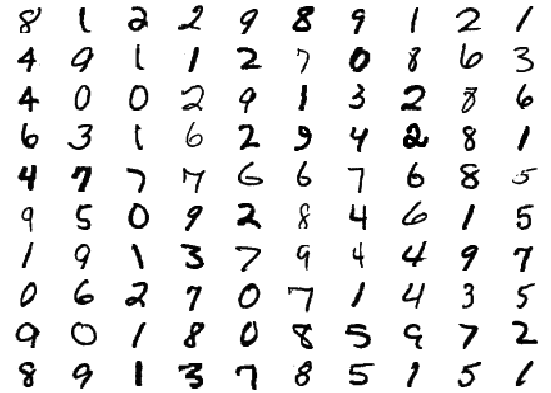
\includegraphics[width=\textwidth]{mnist_data_examples}
    \caption{Example of 100 randomly chosen digits from the MNIST train set.}
    \label{fig:mnist_data_examples}
\end{figure}

The MNIST dataset was used in the article \citetitle{Gal2016Active} by \citeauthor{Gal2016Active} to compare the performance of Bayesian CNNs with frequentist CNNs in the context of Active Learning. This experiment was replicated in this work by using the same architecture that was explained in the article.

The experiment consists in starting with a random but balanced sample of 20 images from the MNIST dataset and acquiring the 10 images that maximize each acquisition function in every iteration, doing 100 acquisition steps for each acquisition function.

The acquisition functions used in the original article are the ones mentioned mentioned in chapter \ref{ch:active_learning}, i.e., Bayesian predictive entropy, frequentist predictive entropy, Bayesian variation ratios, frequentist variation ratios, BALD, random, and an additional one called ``Mean STD'' which was not implemented in this work because of its bad performance in the original article.

The architecture of the neural network used to train the model convolution-relu-convolution-relu-max pooling-dropout-dense-relu-dropout-dense-softmax, with 32 convolution kernels, $4 \times 4$ kernel size, $2 \times 2$ pooling, dense layer with 128 units, and dropout probabilities $0.25$ and $0.5$. For the Bayesian acquisition functions, the posterior predictive distribution samples were obtained by using the dropout trick mentioned in chapter \ref{ch:ann}.

The results can be seen in figure \ref{fig:mnist_comparison_active_learning_random}, where the results of our implementation are on the left and the original article's results are shown on the right. Our implementation achieved the goal of outperforming a random acquisition function, but the results differ when one compares the Bayesian and the frequentist approach. The article's authors claim that the use of a Bayesian approach in the acquisition process of Active Learning leads to better accuracy with fewer images, but in our implementation this does not happen.

This can be seen with more detail in figures in \ref{fig:mnist_pred_entropy_AL} and \ref{fig:mnist_var_ratios_AL} that show our results on the left and the article's results on the right. In the article, the frequentist acquisition functions show a worse performance than their Bayesian counterparts, while in our implementation there is virtually no distinction. For example, with predictive entropy in figure \ref{fig:mnist_pred_entropy_AL}, the frequentist acquisition function in the original article achieve a 90\% accuracy with around 300 images, while in our implementation this accuracy is first achieved with around 200 images.

\begin{figure}[H]
    \centering
    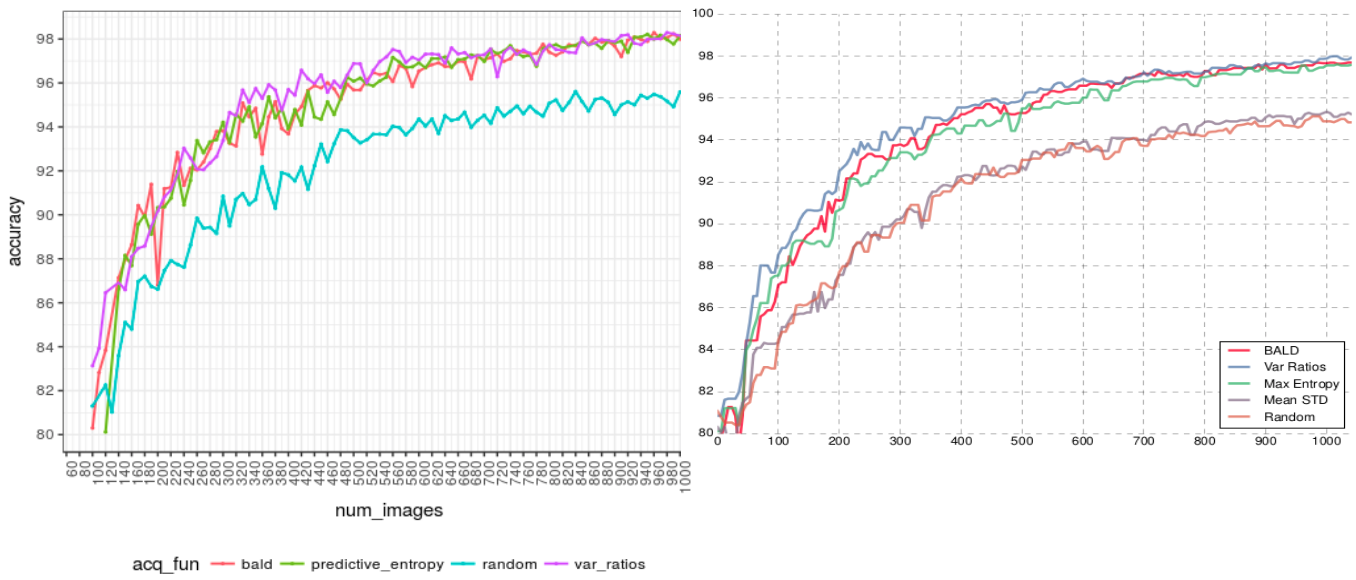
\includegraphics[width=\textwidth]{mnist_bayesian_accuracy.png}
    \caption{Accuracy of models in each acquisition step. The left picture shows our implementation and the right picture shows \citeauthor{Gal2016Active}'s implementation.}
    \label{fig:mnist_comparison_active_learning_random}
\end{figure}

\begin{figure}[H]
  \centering
  \subfloat[Our results.]{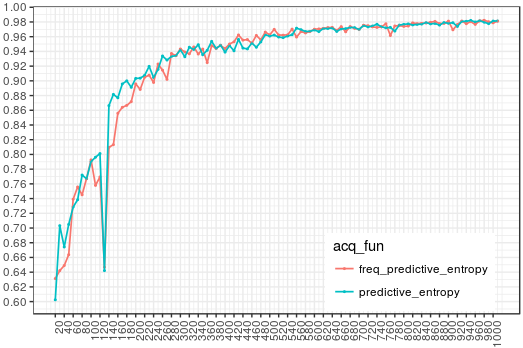
\includegraphics[width=0.5\textwidth]{mnist_pred_entropy_mine.png}}
  \hfill
  \subfloat[Paper's results.]{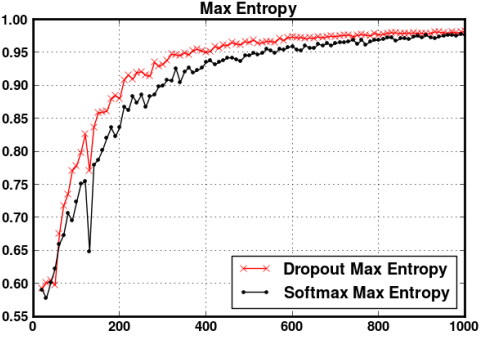
\includegraphics[width=0.5\textwidth]{mnist_pred_entropy_islam.png}}
  \caption{Accuracy of Bayesian and frequentist models in each acquisition step using predictive entropy as acquisition function. The left picture shows our implementation and the right picture shows \citeauthor{Gal2016Active}'s implementation.}
  \label{fig:mnist_pred_entropy_AL}
\end{figure}


\begin{figure}[H]
  \centering
  \subfloat[Our results.]{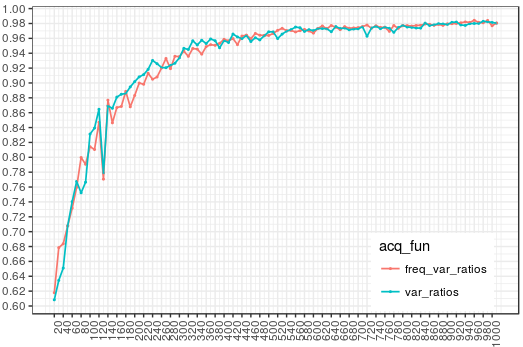
\includegraphics[width=0.5\textwidth]{mnist_var_ratio_mine.png}}
  \hfill
  \subfloat[Paper's results.]{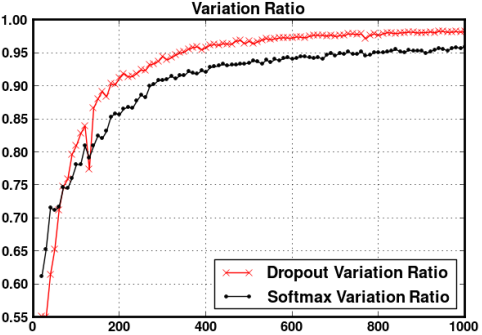
\includegraphics[width=0.5\textwidth]{mnist_var_ratio_islam.png}}
  \caption{Accuracy of Bayesian and frequentist models in each acquisition step using variation ratios as acquisition function. The left picture shows our implementation and the right picture shows \citeauthor{Gal2016Active}'s implementation.}
  \label{fig:mnist_var_ratios_AL}
\end{figure}


% One more thing that should be mentioned is that I could not implement the BALD acquisition in the frequentist setting because of the way it is defined. The BALD uncertainty for a prediction $y$ given model parameters $\mathcal{W}$, features $x$ and training data $\mathcal{D}$ is defined as
%
% \begin{equation}
% 	\label{eq:bald_def}
% 	\mathbb{I}[y, \mathcal{W} | x, \mathcal{D}] = \mathbb{H}[y | x, \mathcal{D}] - \mathbb{E}_{p(\mathcal{W} | \mathcal{D})}[\mathbb{H}[y | x, \mathcal{W}]]
% \end{equation}
%
% with $\mathbb{H}[y | x, \mathcal{D}]$ is the predictive entropy and is defined as $-\sum_c p(y = c | x, \mathcal{D}) \log p(y = c | x, \mathcal{D})$. In the Bayesian case, we have a set of $T$ dropout samples that approximate the predictive distribution, so the second part of equation \ref{eq:bald_def}, i.e., the expected value $\mathbb{E}_{p(\mathcal{W} | \mathcal{D})}[\mathbb{H}[y | x, \mathcal{W}]]$ is approximated by averaging the predictive entropy of each predictive sample; this way $\mathbb{I}[y, \mathcal{W} | x, \mathcal{D}]$ is computed by taking the difference of this quantity and the first part of equation \ref{eq:bald_def}. In the frequentist case, we only have one point estimate, so that difference is zero, so $\mathbb{I}[y, \mathcal{W} | x, \mathcal{D}]$ is zero for all points in the pool set. To this day, I don't know how the paper's authors computed it because their Github code is not clear and they haven't answered my email where I asked them that.

\section{Cats and dogs dataset}


\begin{figure}[H]
    \centering
    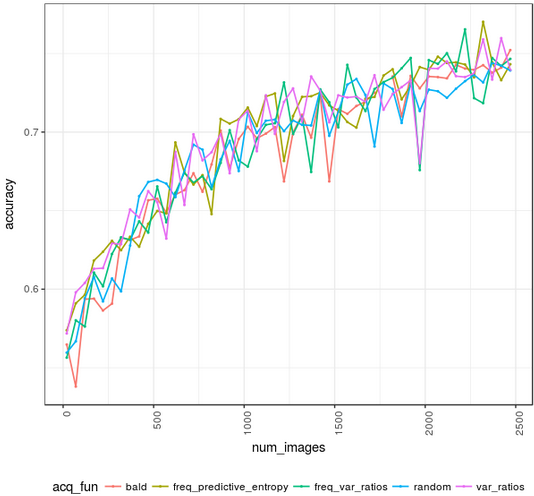
\includegraphics[width=\textwidth]{cats_dogs_accuracy.png}
    \caption{Accuracy of models in each acquisition step in the cats and dogs dataset.}
    \label{fig:cats_dogs_comparison_active_learning_random}
\end{figure}


\section{CIFAR-10 dataset}

\begin{figure}[H]
    \centering
    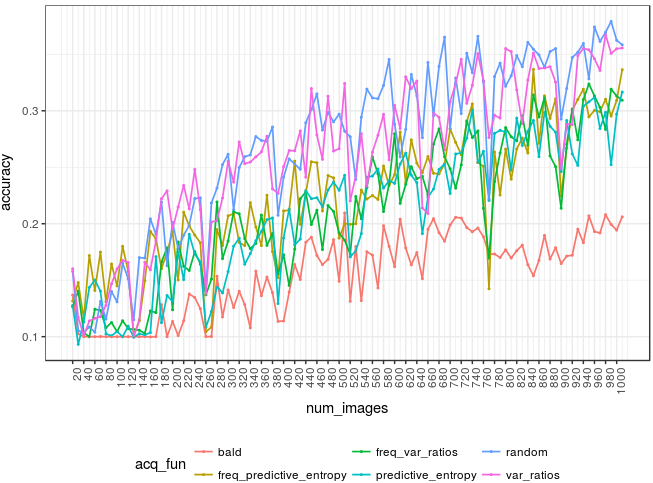
\includegraphics[width=\textwidth]{cifar10_accuracy.png}
    \caption{Accuracy of models in each acquisition step in the CIFAR-10 dataset.}
    \label{fig:cifar10_comparison_active_learning_random}
\end{figure}

\section{Discussion}

\begin{figure}[H]
    \centering
    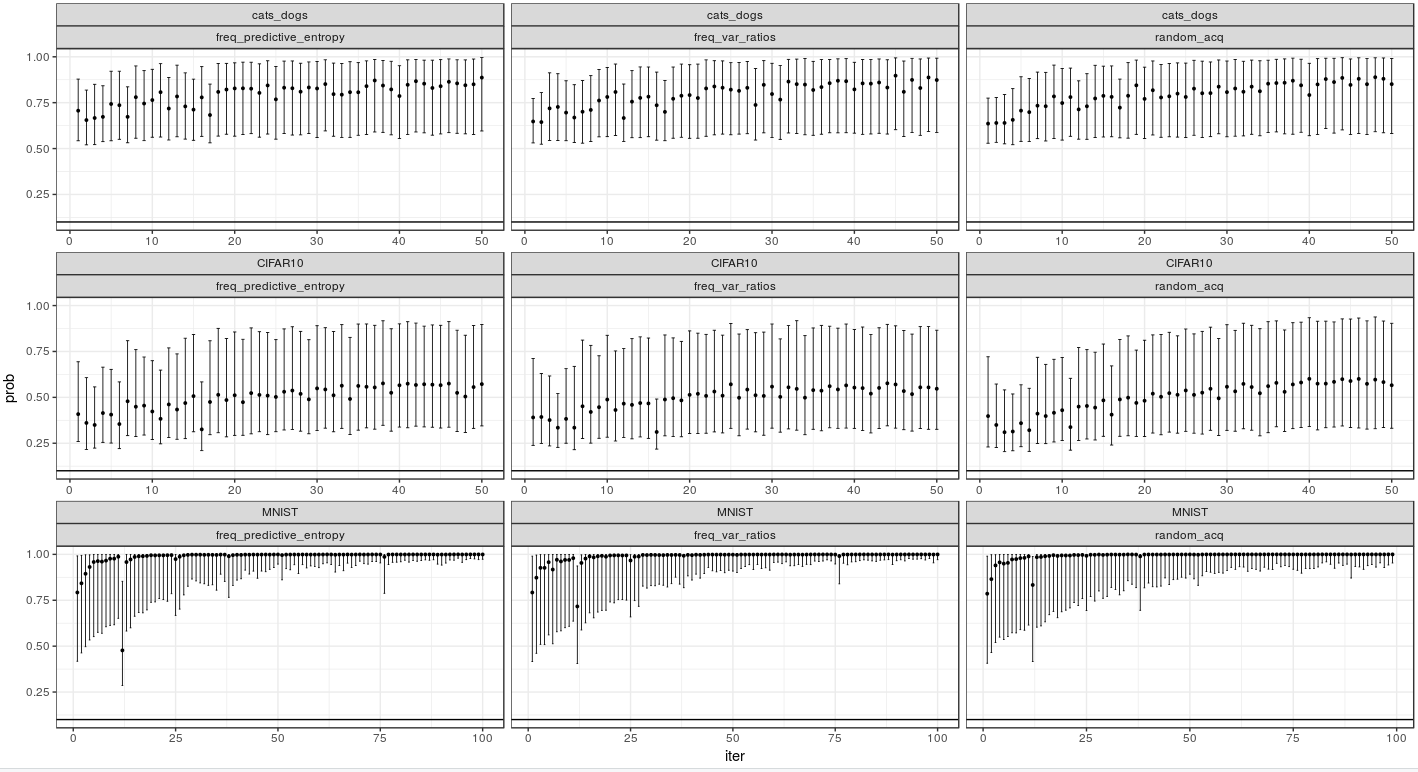
\includegraphics[width=\textwidth]{probs_iterations.png}
    \caption{Probabilities of each model in each acquisition iteration.}
    \label{fig:probs_iterations}
\end{figure}
